%keep
%5
%6
%9
% 1/2 10 + 1/2 12
%14
%16, edited

%cut
%2, 3, 7, 8
%%%%%%%%%%%% BEGIN PREAMBLE 
\documentclass[handout, serif]{beamer}
%\usepackage[T1]{fontenc}
\usepackage[utf8]{inputenc}
\usepackage{biolinum}
\usepackage{mathtools}
\setbeamertemplate{bibliography item}[text]
\usepackage{microtype}
\usepackage{bm}
\usepackage{amssymb}
\usepackage{wasysym}
\usepackage{mathrsfs}
\usepackage{setspace,tikz,xcolor,listings,multicol}
\usepackage{ragged2e}
\usetikzlibrary{arrows,matrix}
\usepackage[vcentermath]{youngtab}
\usepackage[english]{babel}
\usepackage[utf8]{inputenc}
\usepackage{tcolorbox}
\usepackage{xcolor}
\newcommand{\arxiv}[1]{\href{http://arxiv.org/abs/#1}{\texttt{arXiv:#1}}}
\definecolor{pink}{RGB}{24, 117, 18}
\definecolor{purple}{RGB}{102, 27, 194}
\definecolor{red}{RGB}{235, 7, 90}
\definecolor{yellow}{RGB}{255, 170, 0}
\newcommand{\ph}{\phantom{.}}
\definecolor{forGreen}{RGB}{0,120,0}
\definecolor{skyBlue}{RGB}{0, 200, 255}
\newcommand{\fgcf}{\scriptsize\color{forGreen}4}
\newcommand{\fgct}{\scriptsize \color{forGreen}2}
\newcommand{\tn}{10}
\DeclareMathOperator{\SD}{SD}
\DeclareMathOperator{\Pt}{P}
\DeclareMathOperator{\sh}{sh}

\usepackage{mathtools}
\usepackage{ytableau}
\usepackage[all]{xy}
\usefonttheme{serif}
\usetheme[nofirafonts]{focus}
\setbeamertemplate{frametitle continuation}{}
\setbeamertemplate{caption}[numbered]
\definecolor{main}{RGB}{0, 75, 135}
\newlength{\myl}
\setlength{\myl}{0.075\linewidth}
\newcommand{\switchyarrowy}{\mathrlap{\curvearrowleft}\hspace{0.09em}\curvearrowright}
\renewcommand{\thempfootnote}{\arabic{mpfootnote}}
\title{The Box-Ball System\\(2020 UCONN REU)}
\institute{\vspace{-3em}BIRS Dynamical Algebraic Combinatorics Workshop}
\date{\vspace{-3em}October 23, 2020}
\begin{document}
\begin{frame}
    \maketitle
      \centering
\vspace{-2em}
  \begin{tabular}{c c c c}
    
\includegraphics[width=.1\linewidth]{Ben.jpeg} &     
\includegraphics[width=.1\linewidth]{Eli.jpeg}  & 
    
\includegraphics[width=.1\linewidth]{Rose.jpeg} &
    
\includegraphics[width=.1\linewidth]{Aubrey.jpeg}\\
    
    \textbf{Ben Drucker} & \textbf{Eli Garcia} & \textbf{Rose Silver} & Aubrey Rumbolt \\
    
\includegraphics[width=\myl]{swarthmore-college-logo.png}&\raisebox{.3em}{
\includegraphics[width=\myl]{Massachusetts_Institute_of_Technology-Logo.wine.png}}&
\includegraphics[width=\myl]{1920px-Northeastern_University_seal.svg.png}&
\includegraphics[width=\myl]{1920px-Seal_of_Western_New_England_University.svg.png}
    \end{tabular}
    
    \centering
\end{frame}
\begin{frame}{Tableaux}
    \begin{block}{Definition. (Young Tableaux)}
        \begin{itemize}
        \small
            \item A Young tableau (pl. tableaux) is an arrangement of numbers $\{1,2,...,n\}$ into rows whose lengths are weakly decreasing.\vspace{-0.25em}
            \item The Young tableau is \textit{standard} if each row is an increasing sequence (going from left to right) and each column is an increasing sequence (going from top to bottom). \vspace{-0.25em}
            % A Young tableau is \textit{nonstandard} if this is not the case.
            \item The \textit{reading word} of a standard Young tableau is the permutation formed by concatenating the rows of the tableau from bottom to top.
        \end{itemize}
    \end{block}
    \begin{exampleblock}{Example. (Standard Young Tableau)}
        \begin{itemize}
        \item \raisebox{-1em}{\tiny \young(12,34,5)} is a standard Young tableau. Its reading word is $53412.$ %PERM: [3, 1, 5, 4, 2]
        \item \raisebox{-1em}{\tiny \young(12,4,5,3)} is a nonstandard Young tableau.
        \end{itemize}
        \vspace{-3.8pt}
    \end{exampleblock}
\end{frame}
\begin{frame}{Robinson-Schensted insertion algorithm}
        \begin{center}
            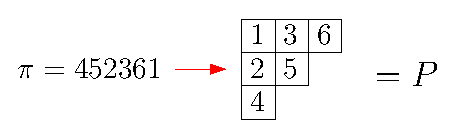
\includegraphics[scale = 0.85]{RS_Example.eps}
        \end{center}
    Let $P$ be the empty tableau. Given a permutation $\pi = \pi_1\cdots\pi_n,$ the \textit{Robinson-Schensted (RS) insertion algorithm} is a method of insertion of each element of $\pi$ into $P.$ The RS insertion algorithm always gives a standard Young tableau.
\end{frame}
    \begin{frame}{Box-Ball System and Example}
A box-ball system is a collection of discrete time states each containing elements of a permutation, $\pi$ in one-line notation. We can move forward in this system by rearranging $\pi$ using the following rule: Place $\pi$ in a strip of infinite boxes. (This corresponds to the $t=0$ state of the system.) Then, move each element of $\pi$ to the nearest empty box to its right, as shown below.
        \pause
        \begin{figure}
            \centering
                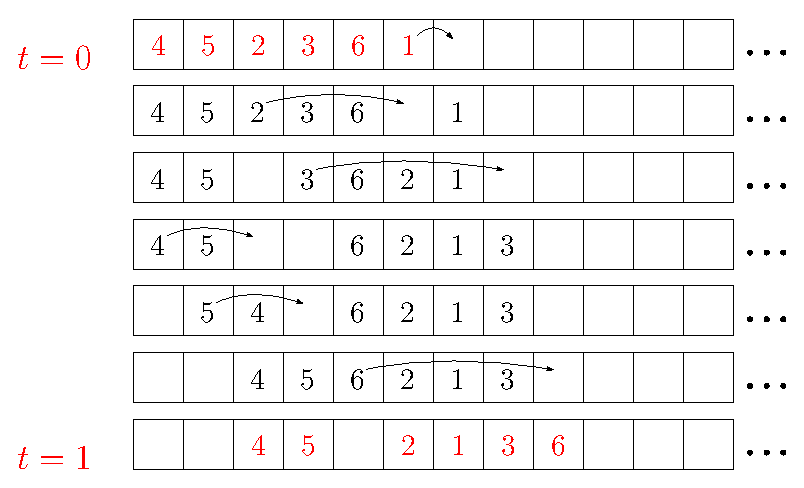
\includegraphics[width = 3in]{Step3.eps}
        \end{figure}
    \end{frame}
    \begin{frame}{Box-Ball System: Example---$\pi=452361$}
        To continue the analysis, keep making BBS moves until we reach a ``steady state" (i.e., the system decomposes into \textit{solitons})
        \begin{figure}
            \centering
            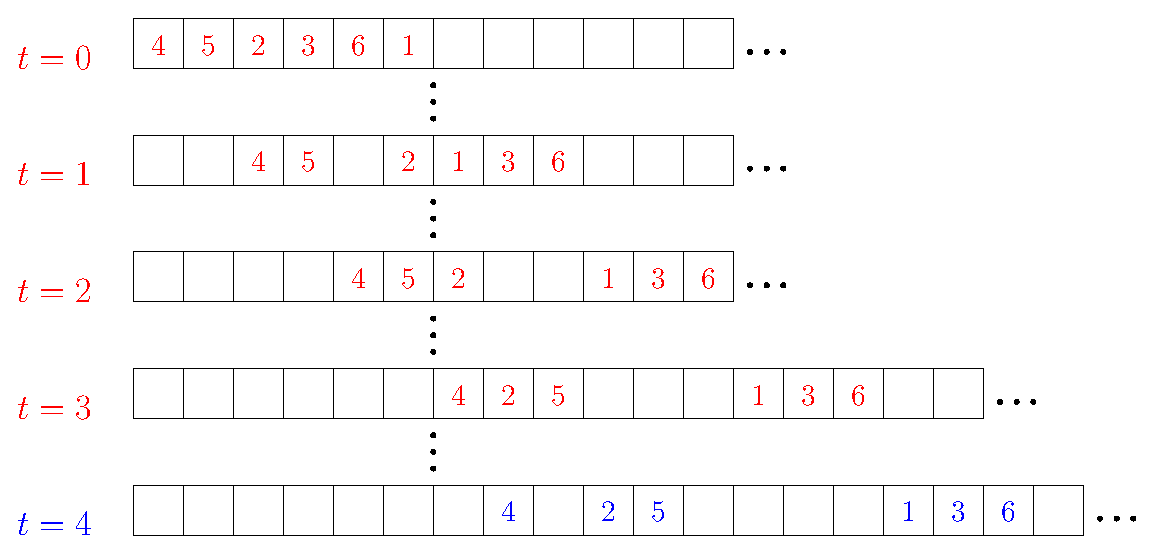
\includegraphics[width = 3in]{Step4V2.eps}
            \end{figure}
        Then, create a (not necessarily standard) tableau by stacking solitons:\\
        \begin{figure}
            \centering
            Soliton decomposition
            ~
            %shape 
            %= 
            \scalebox{0.7}{$\young(136,25,4)$} with shape $(3,2,1)$.
        \end{figure}
\end{frame}
\begin{frame}{Selected Results Involving Tableaux}
     \begin{alertblock}{Theorem}
        The following are equivalent: \begin{enumerate}
            \item $\SD(\pi) = \Pt(\pi).$
            \item $\SD(\pi)$ is a standard tableau.
        \end{enumerate}
    \end{alertblock}
    \begin{block}{Conjecture}
        The following is equivalent to (1) and (2).
        \begin{enumerate}
            \setcounter{enumi}{2}
            \item $\sh\SD(\pi) = \sh\Pt(\pi).$ 
        \end{enumerate}
    \end{block}
    \begin{itemize}
        \item We have shown $(1)\Longleftrightarrow(2)$ and $(1) \implies (3).$ It remains to prove $(3)\implies(1).$
    \end{itemize}
\end{frame}
\begin{frame}{Selected Results Involving Steady-State Times}
    \begin{alertblock}{Theorem: Classification of permutations with steady-state value of $t=0$}
    A permutation $r$ has a box-ball steady-state value of $t=0$ if and only if $r$ is the reading word of a standard tableau.
    \end{alertblock}
    \begin{alertblock}{Theorem: Some permutations with steady-state value of $t=1$}
     Let $r$ be the reading word of a standard tableau $P$. If $r'$ is the permutation resulting from the swapping of a special pattern of elements in $r$, then $r'$ has a box-ball steady-state value of $t=1.$ ($r'$ is the result of performing a \textit{Knuth move} on $r$.)
    \end{alertblock}
    \small
    \begin{block}{$n-3$ conjecture}
        The steady-state time for a permutation in $S_n$ is no more than $n-3.$
    \end{block}
\end{frame}
\begin{frame}[focus]
        Thank You! \\
        Questions?
\end{frame}
\end{document}